\documentclass[crop,tikz]{standalone}
\usepackage{amsmath}
\usetikzlibrary{arrows}
\usetikzlibrary{positioning}
\usetikzlibrary{shapes}
\usetikzlibrary{hobby}
\usepackage[draft]{tikzpeople}

\newcommand\irregularcircle[2]{% radius, irregularity
  +(0:{(#1)+rand*(#2)})
  \foreach \a in {10,20,...,350}{
    -- +(\a:{(#1)+rand*(#2)})
  } -- cycle
}

\begin{document}
\begin{tikzpicture}
  \tikzset{line/.style={draw, <->, >=latex'}}
  \tikzset{line2/.style={draw, ->, >=latex'}}
  \tikzset{line3/.style={draw, <->, >=latex', dashed}}

  \node[] at (0,0)
  {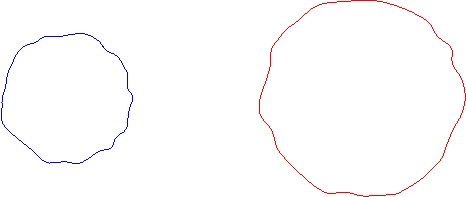
\includegraphics[width=\textwidth]{./figure-state-draw}};

  \draw [fill=black] (-5, 0.8) node[below left] {\{\}} circle (2pt);
  \draw [fill=black] (3, 1)  node[above right] {\{\}} circle (2pt);
  \path (-5, 0.8) edge[bend left=15, line3, thick] node[pos=0.55,
  above] {create\_account() $\rightarrow$ A} (3, 1);

\end{tikzpicture}
\end{document}